Nous allons étudier la robustesse du système par rapport au nombre de personne,
le bruit, l'inversion du contraste, la rotation et la translation.


\subsection{Robustesse au nombre de personnes}
Nous avons déjà dit lorsque nous avons présenté nos résultats que quand il y a
40 personnes, le taux de reconnaissance est de $68\%$, alors que quand
il y a 20 personnes, celui-ci est de $82\%$. Ce large écart nous pousse à étudier
l'influence que peut avoir le nombre de personnes sur les performances du système.

La figure \ref{fig:robustness:nombre_de_personnes} montre l'évolution du taux
de reconnaissances correctes en fonction du nombre de personnes.

\begin{figure}[H]
    \centering
    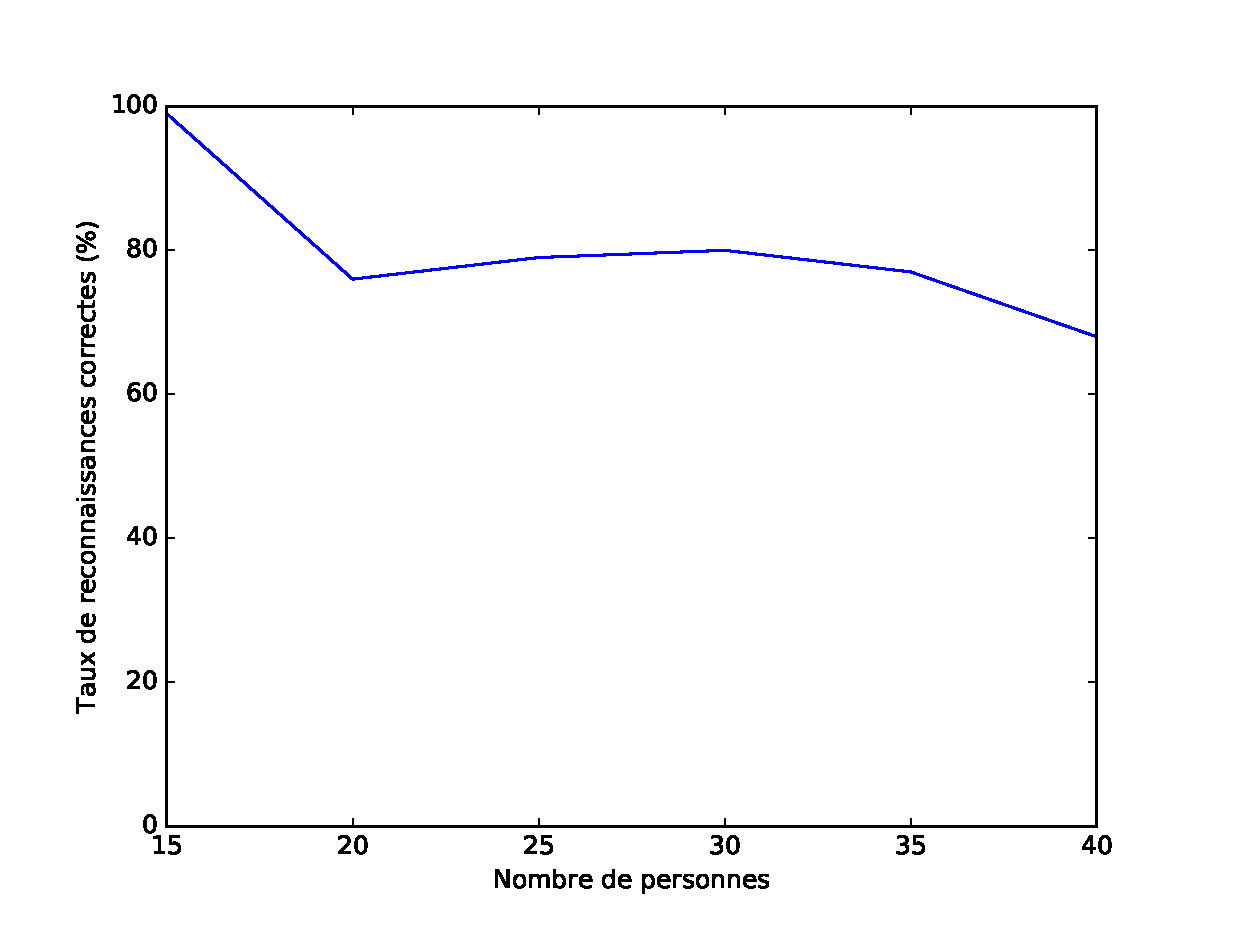
\includegraphics[scale=0.5]{images/robustesse_nombre_de_personnes}
    \caption{Taux de reconnaissance en fonction du nombre de personnes.}
    \label{fig:robustness:nombre_de_personnes}
\end{figure}
On voit que ça suit une tendance baissière assez faible, restant dans la 
marge des $70\%-80\%$.
Malheureusement, comme il y a 40 personnes dans la base de données AT\&T, on ne 
peut pas tester pour des valeurs supérieures à 40.


\subsection{Robustesse au bruit}
\subsubsection{Bruit blanc gaussien}
On entraîne le système sur des données non bruitées puis on le teste sur des images
bruitées. La figure \ref{fig:robustness:gaussien:test} montre les variations du taux
de reconnaissances correctes en fonction de la variance $\sigma^2$ du bruit blanc
gaussien.
\begin{figure}[H]
    \centering
    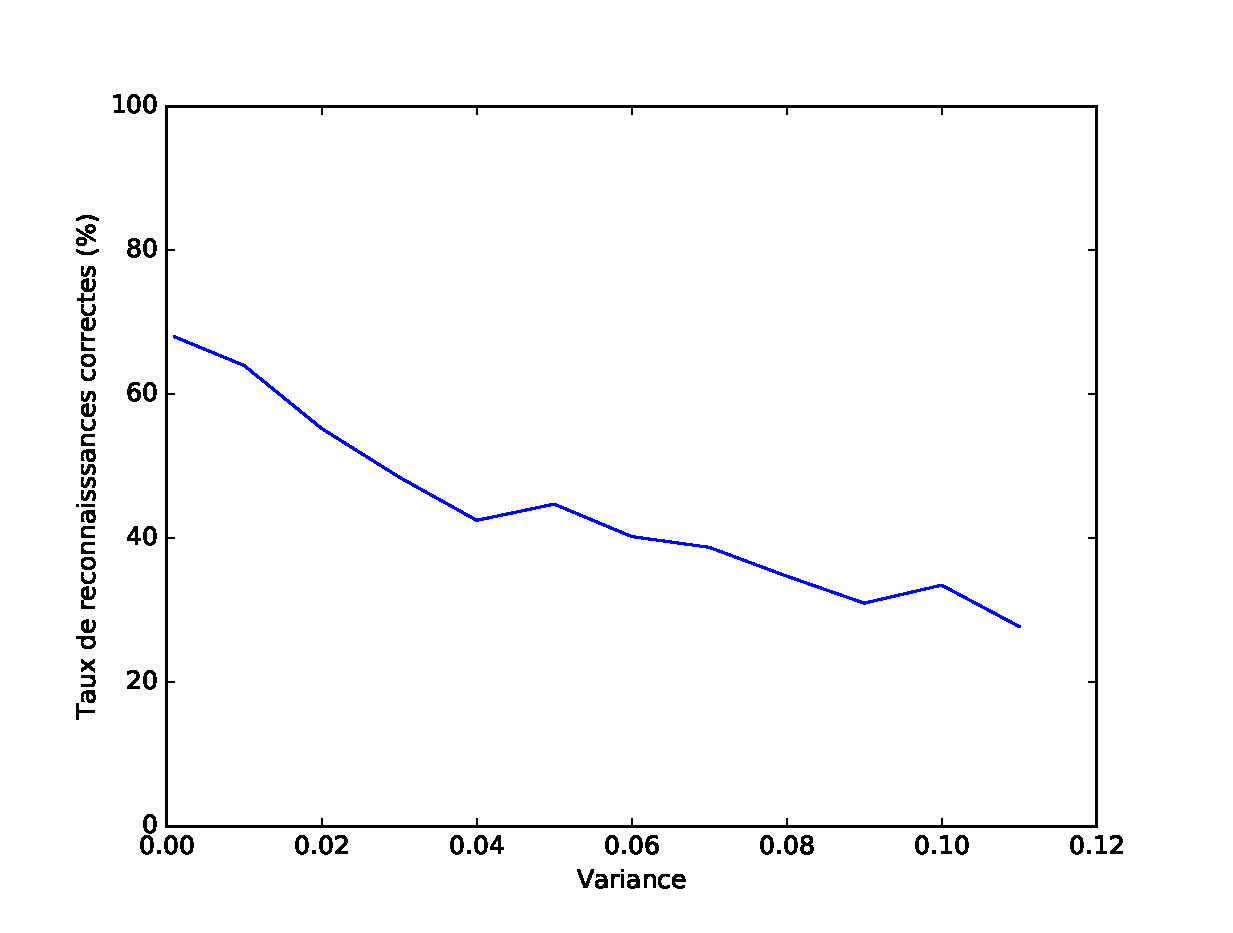
\includegraphics[scale=0.5]{images/robustesse_gaussien_test}
    \caption{Taux de reconnaissance en fonction de la variance du bruit blanc gaussien
    (apprentissage sur des images non bruitées).}
    \label{fig:robustness:gaussien:test}
\end{figure}
Pour mieux visualiser la chose, la figure \ref{fig:robustness:gaussien:exemple} montre
une image non bruitée et la même image avec des bruits gaussiens de différentes variances.
\begin{figure}[H]
    \centering
    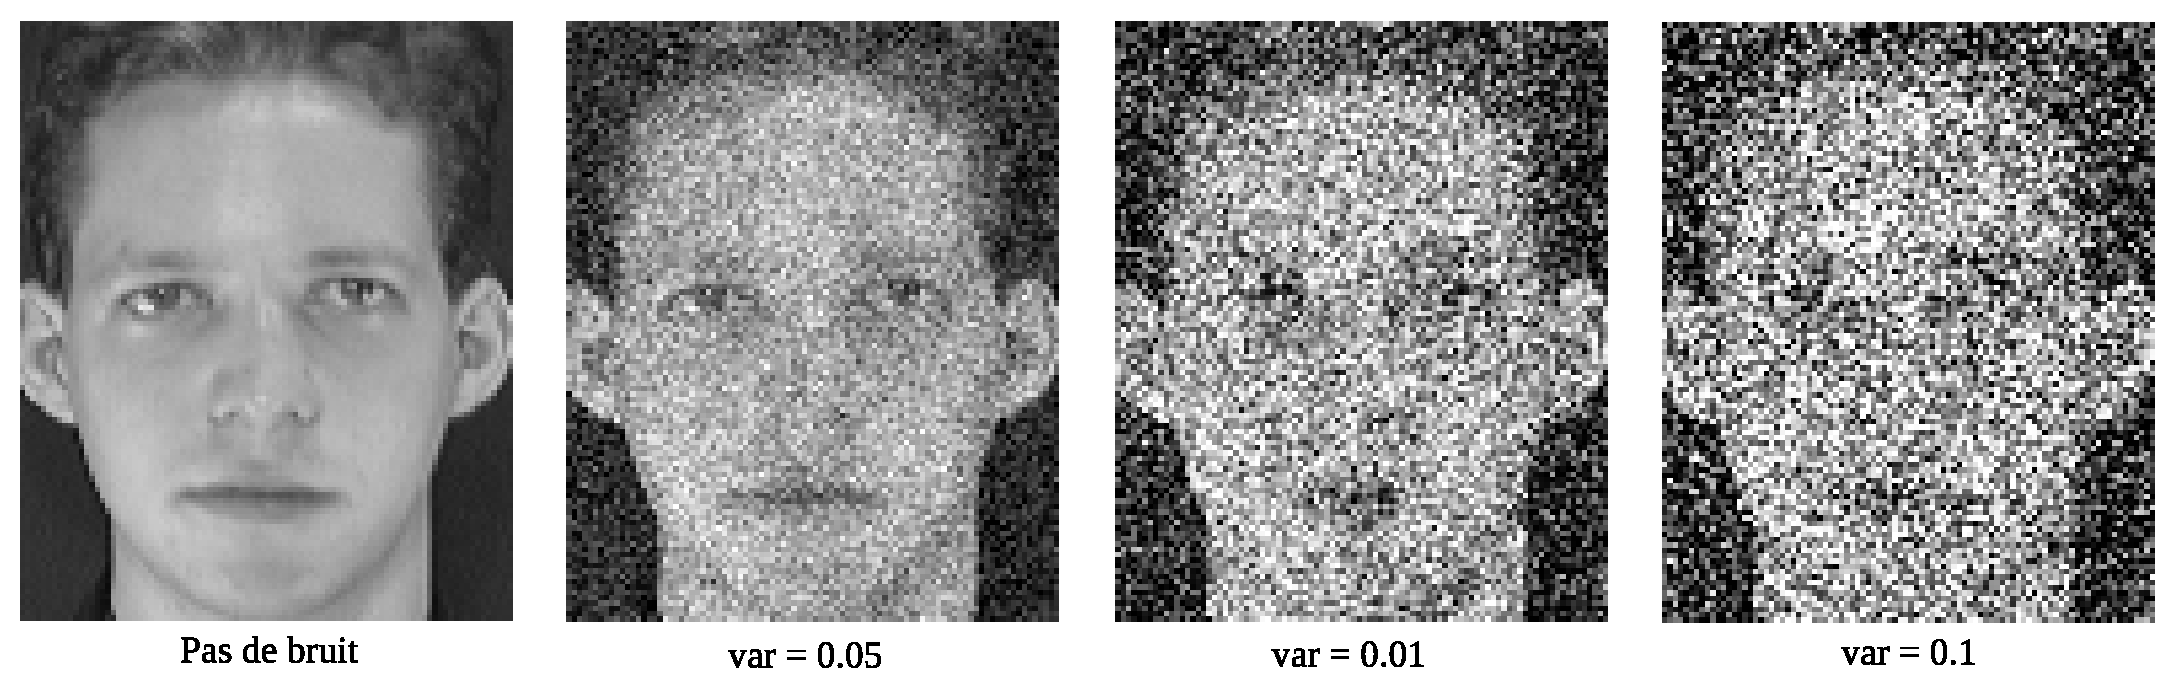
\includegraphics[scale=0.44]{images/robustness_gaussien_exemple}
    \caption{Exemple de bruits blancs gaussiens de différentes variances.}
    \label{fig:robustness:gaussien:exemple}
\end{figure}
Nous voyons que les performances commencent à décroître dès que le bruit
devient apparent. Pour une variance supérieure à $0.1$, on n'attend pas du système
qu'il ait de bonnes performances car même un être humain aurait des difficultés à
reconnaître la personne.

Maintenant, au lieu d'entraîner sur des données non bruitées et de tester sur des 
données bruitées, nous allons introduire un pourcentage ($30\%$) d'images bruitées
dans les images d'entraînement et de test. Le graphe de la figure \ref{fig:robustness:gaussien:tout} 
montre les taux de reconnaissance obtenus pour différentes variances.
\begin{figure}[H]
    \centering
    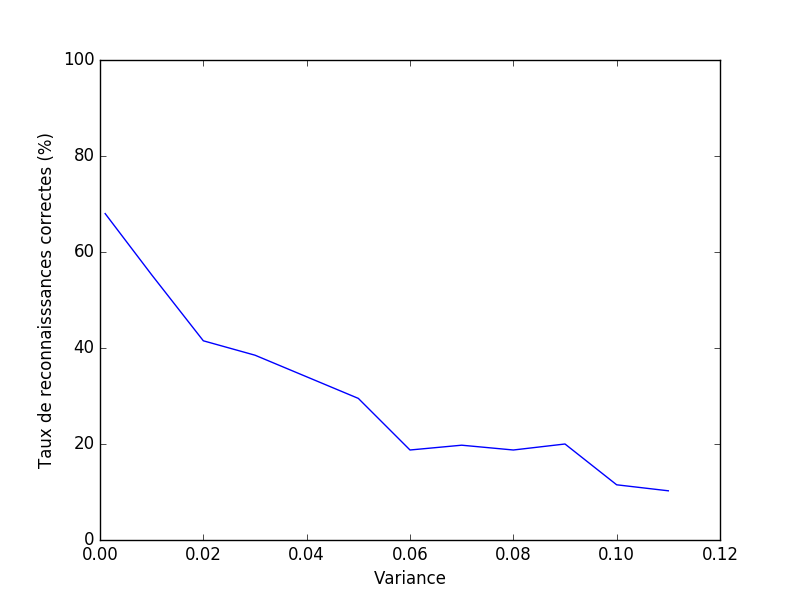
\includegraphics[scale=0.5]{images/robustesse_gaussien_tout}
    \caption{Taux de reconnaissance en fonction de la variance du bruit blanc gaussien
    (apprentissage sur des images bruitées).}
    \label{fig:robustness:gaussien:tout}
\end{figure}
Les performances cette fois-ci sont inférieures à celles que nous avions obtenu lorsque nous
avons utilisé uniquement des données non bruitées pour l'entraînement. Nous suspectons que 
l'introduction de bruits dans les données d'entraînement a conduit à une mauvaise reconnaissance
des images non bruitées (en plus des images bruitées).

On conclue que le système est peu robuste aux bruits gaussiens. 
Ces résultats sont toutefois à prendre avec
précaution étant donné le nombre limité d'images disponibles.

\subsubsection{Bruit de Poisson}
La figure \ref{fig:robustness:poisson} montre une image avant et après application d'un bruit de Poisson.
Après avoir entraîné le système sur des images non bruitées, quand on teste sur des images
bruitées (bruit de Poisson), le taux de reconnaissances correctes est de $68\%$, le même que
sur des données non bruitées. On en conclue que le système est robuste aux bruits de Poisson.
\begin{figure}[H]
    \centering
    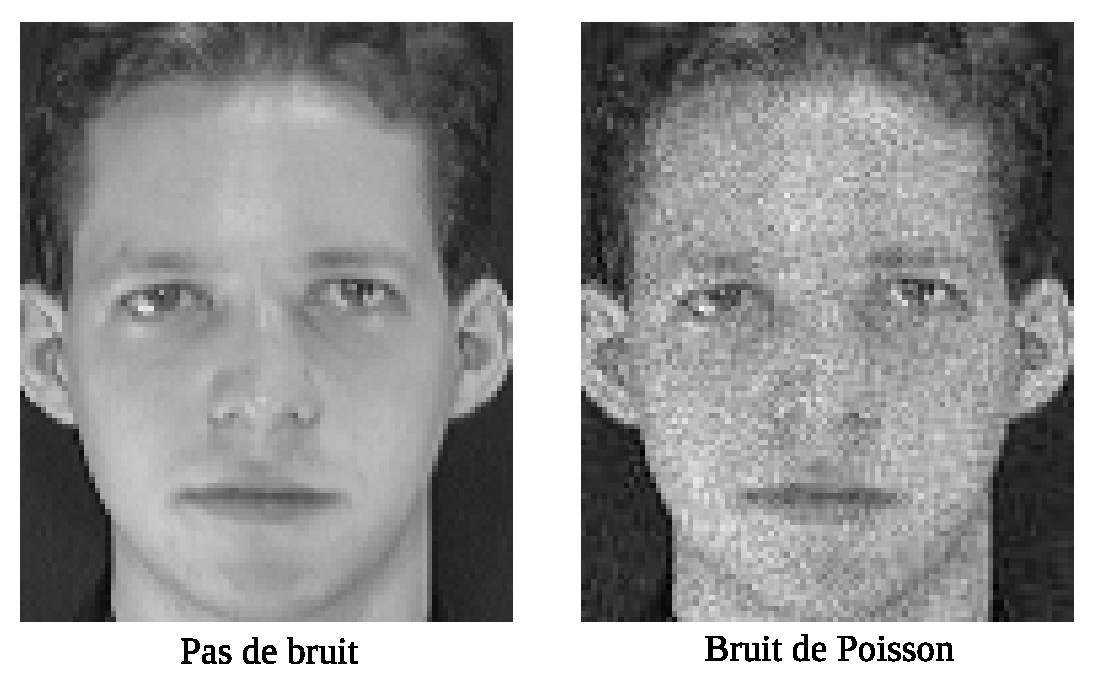
\includegraphics[scale=0.6]{images/exemple_poisson}
    \caption{Exemple d'un bruit de Poisson.}
    \label{fig:robustness:poisson}
\end{figure}

\subsubsection{Bruit Speckle}
On entraîne le système sur des données non bruitées puis on le teste sur des images
bruitées. La figure \ref{fig:robustness:speckle:test} montre les variations du taux
de reconnaissances correctes en fonction de la variance $\sigma^2$ du bruit speckle.
\begin{figure}[H]
    \centering
    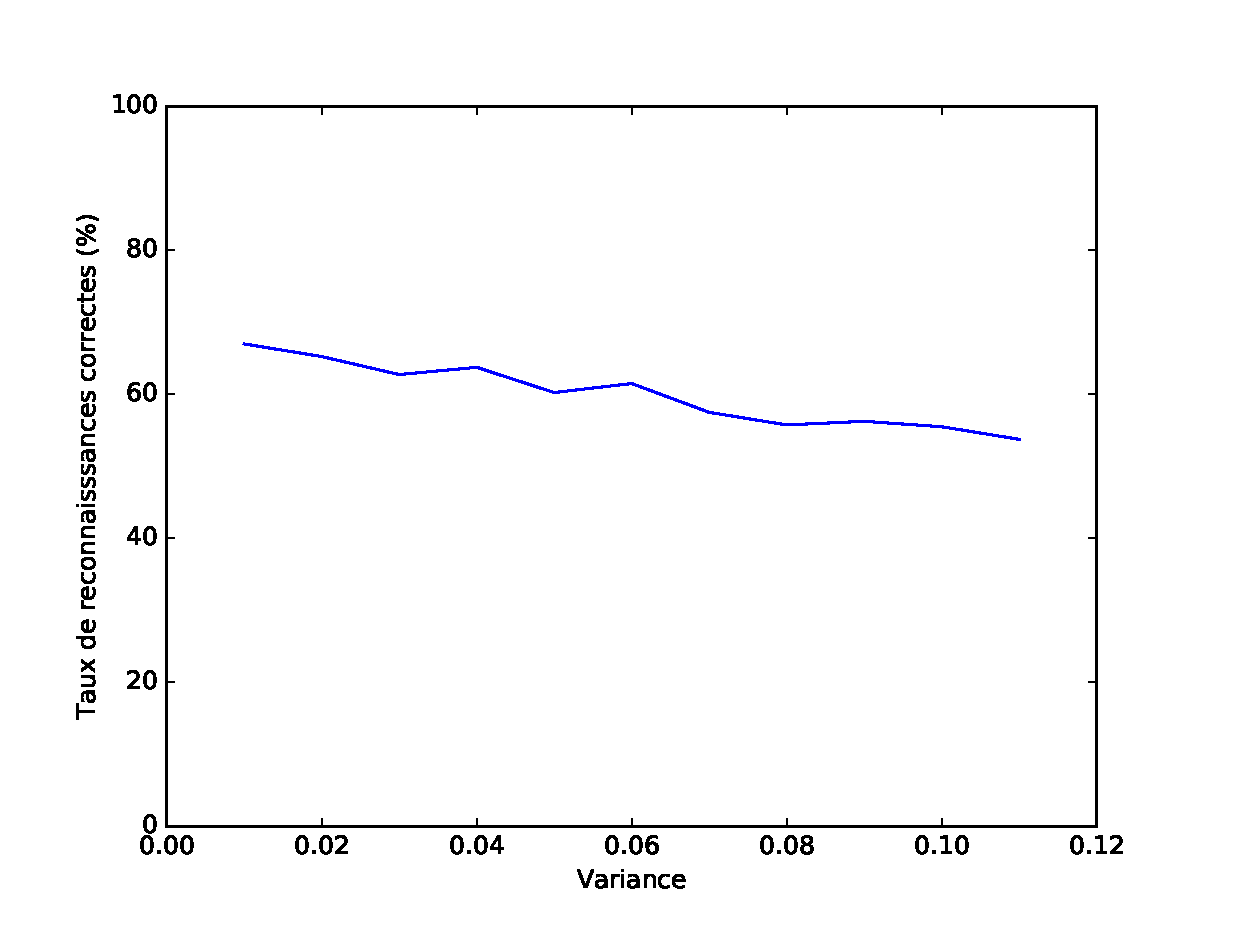
\includegraphics[scale=0.5]{images/robustesse_speckle_test}
    \caption{Taux de reconnaissance en fonction de la variance du bruit speckle.}
    \label{fig:robustness:speckle:test}
\end{figure}
Pour mieux visualiser la chose, la figure \ref{fig:robustness:speckle:exemple} montre
une image non bruitée et la même image avec des bruits speckle de différentes variances.
\begin{figure}[H]
    \centering
    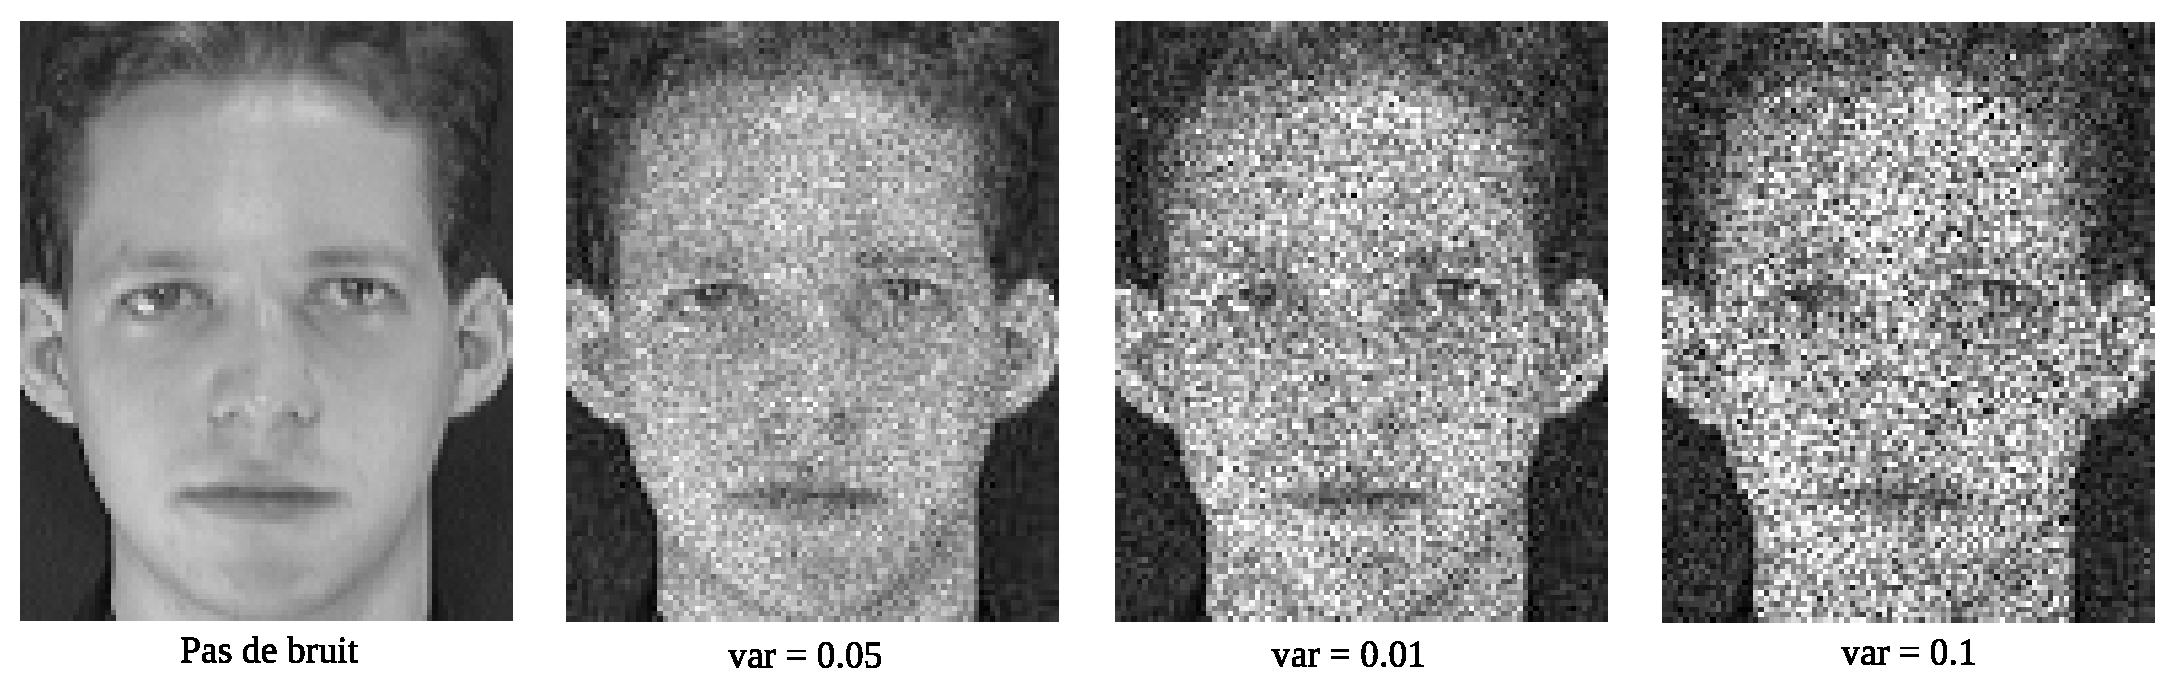
\includegraphics[scale=0.44]{images/robustness_speckle_exemple}
    \caption{Exemple de bruits speckle de différentes variances.}
    \label{fig:robustness:speckle:exemple}
\end{figure}

Nous voyons qu'il y a une détérioration des performances à mesure que le bruit speckle
devient apparent, mais le système conserve quand-même un taux de reconnaissance assez 
satisfaisant (comparé à ses performances dans le cas sans bruits). On en conclue que le
système est assez robuste au bruit speckle (Il n'est pas totalement robuste, ses performances
diminuent là où celles d'un être humain resteraient les mêmes).

\subsubsection{Bruit poivre et sel}
On entraîne le système sur des données non bruitées puis on le teste sur des images
bruitées. La figure \ref{fig:robustness:sp:test} montre les variations du taux
de reconnaissances correctes en fonction du pourcentage des pixels de l'image affectés
par le bruit poivre et sel.
\begin{figure}[H]
    \centering
    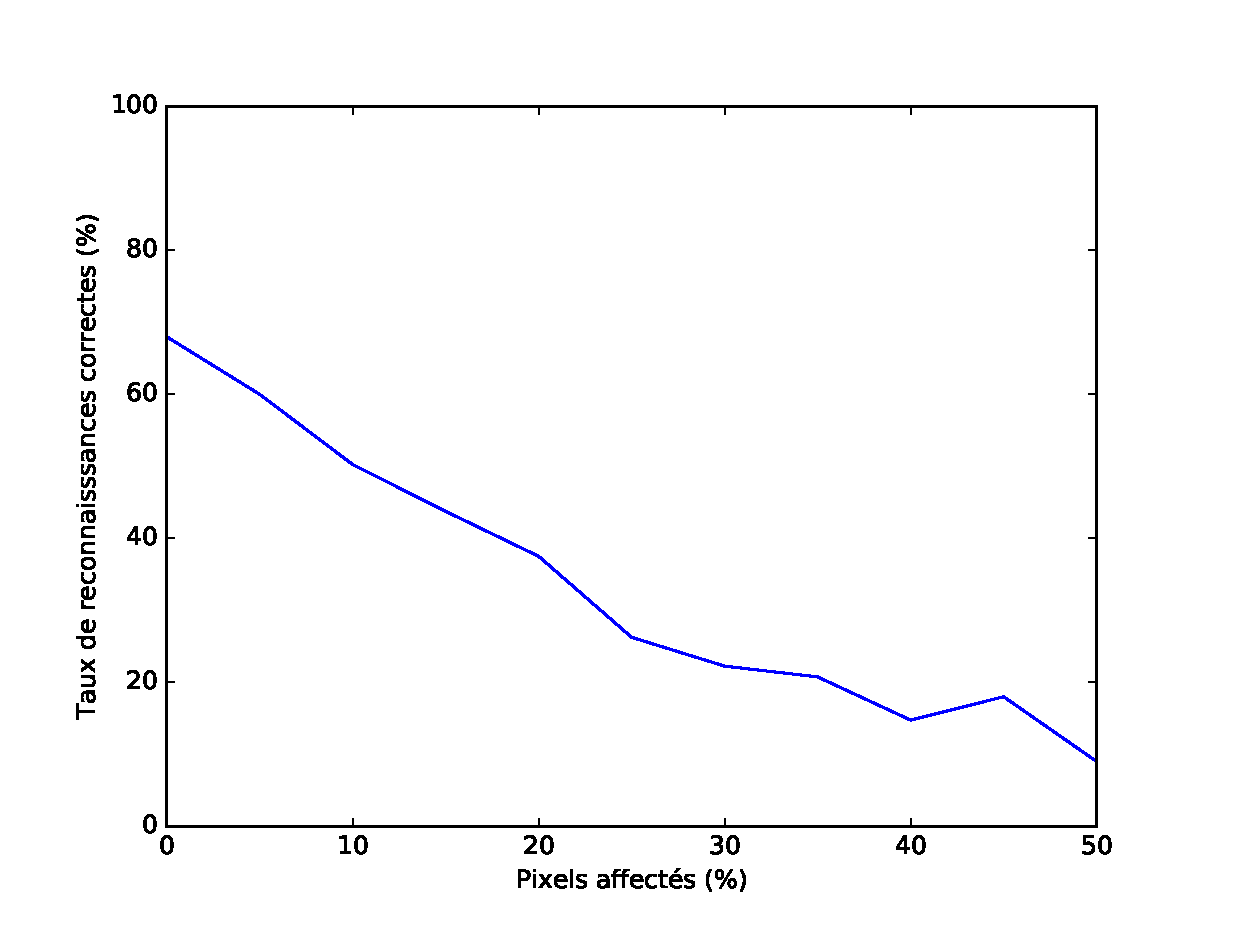
\includegraphics[scale=0.5]{images/robustesse_sp_test}
    \caption{Taux de reconnaissance en fonction du pourcentage des pixels bruités
    (bruit poivre et sel, apprentissage sur des images non bruitées).}
    \label{fig:robustness:sp:test}
\end{figure}
Pour mieux visualiser la chose, la figure \ref{fig:robustness:sp:exemple} montre
une image non bruitée et la même image avec des bruits poivre et sel affectant 
différents pourcentages de pixels.
\begin{figure}[H]
    \centering
    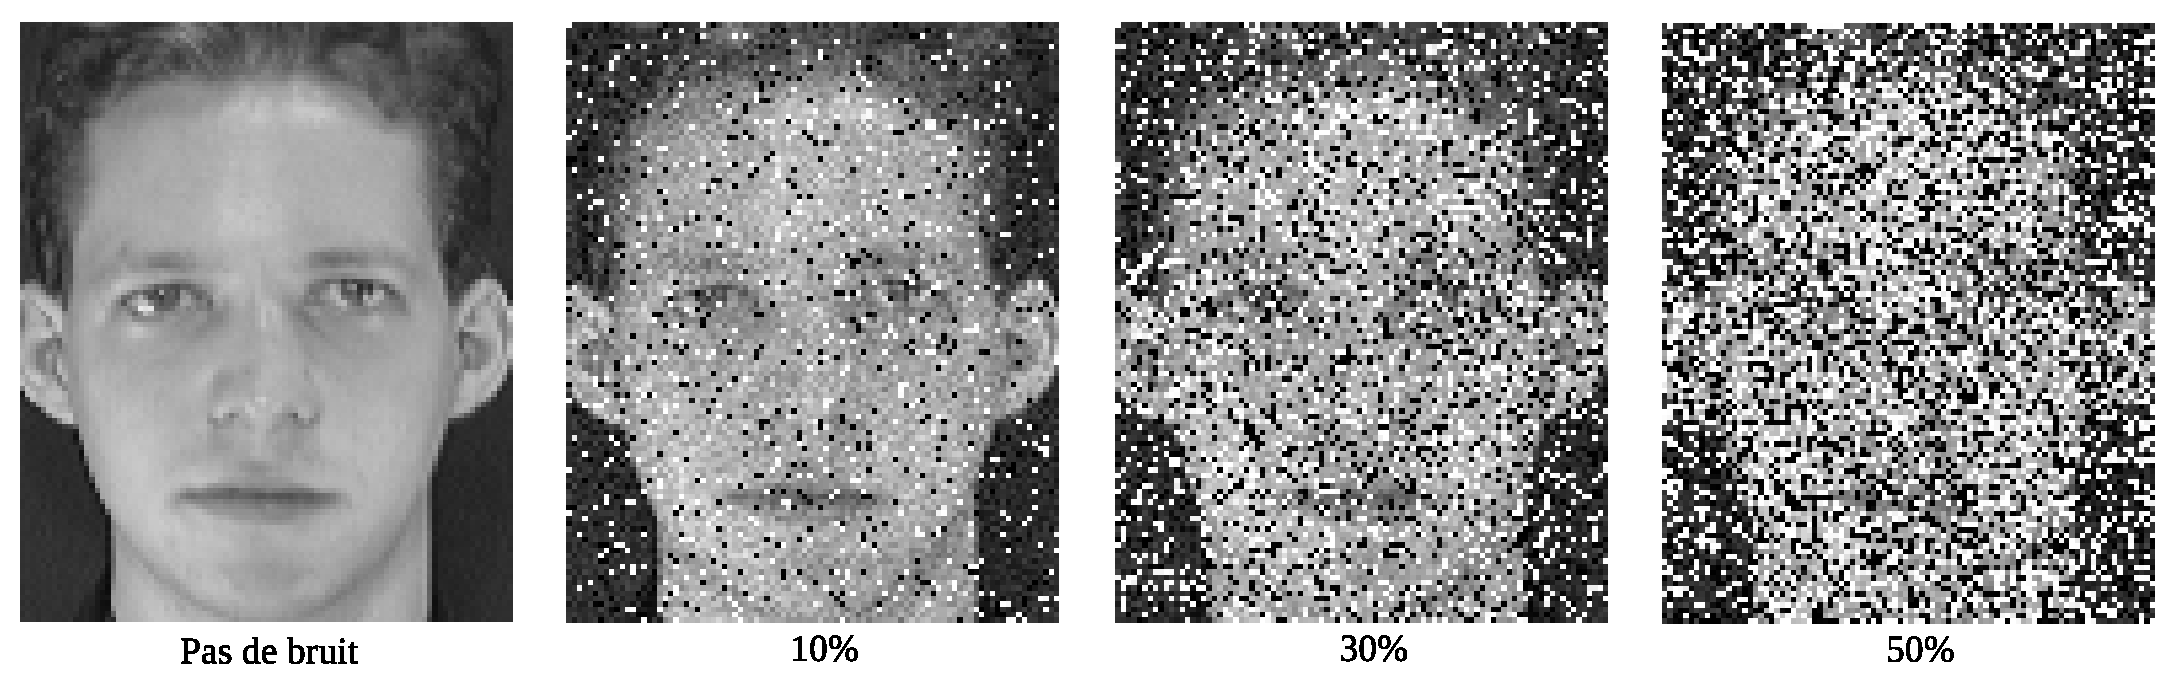
\includegraphics[scale=0.44]{images/robustness_sp_exemple}
    \caption{Exemple de bruits poivre et sel affectant différents pourcentages de pixels.}
    \label{fig:robustness:sp:exemple}
\end{figure}

Nous voyons que les performances commencent à décroître dès que le bruit
devient apparent, donc à la base, le système n'est pas robuste aux bruits
poivre et sel.

Maintenant, au lieu d'entraîner sur des images non bruitées et de tester sur des 
images bruitées, nous allons introduire un pourcentage ($30\%$) d'images bruitées
dans les images d'entraînement et de test. Le graphe de la figure \ref{fig:robustness:sp:tout} 
montre les taux de reconnaissance obtenus pour différents pourcentages de pixels affectés.
\begin{figure}[H]
    \centering
    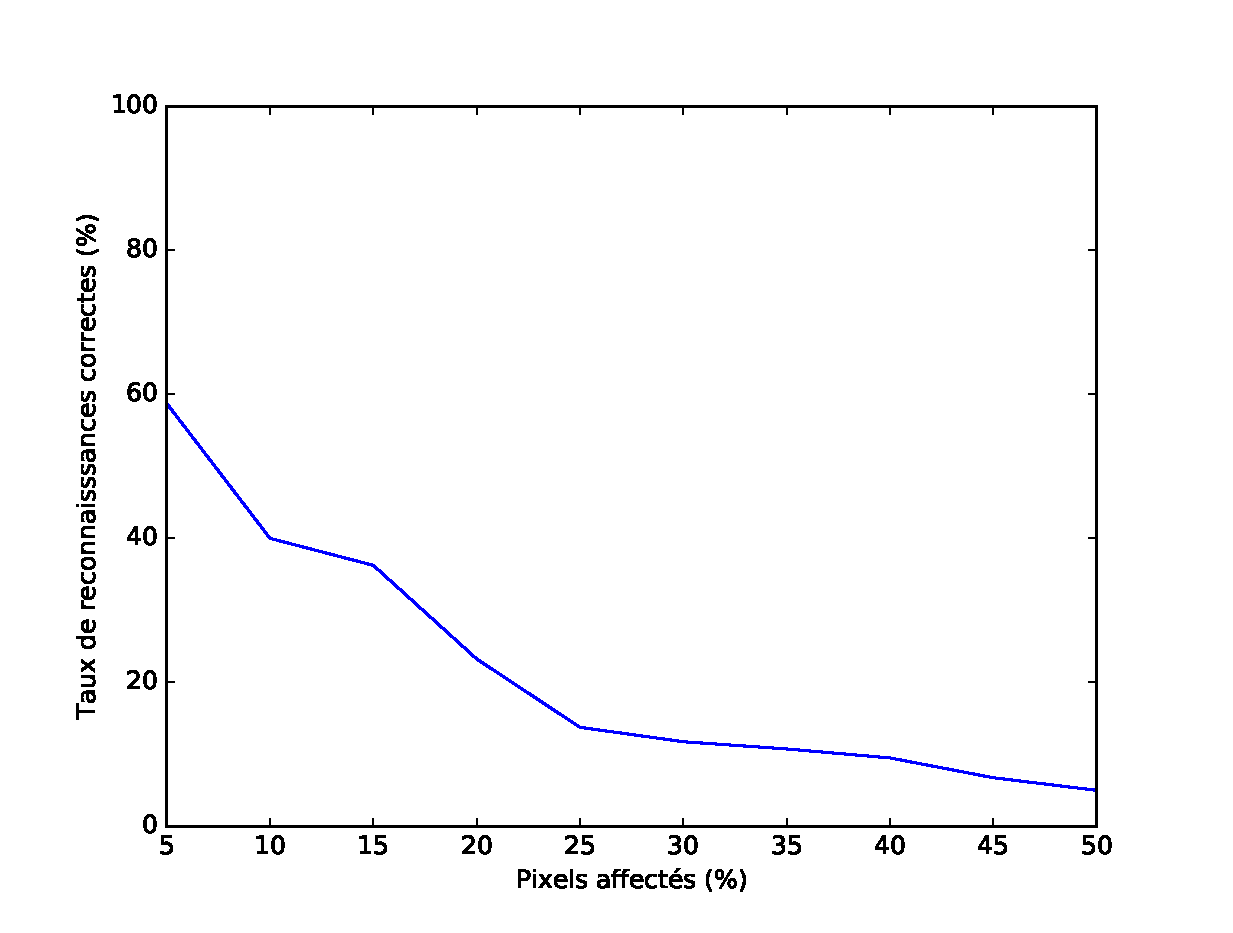
\includegraphics[scale=0.5]{images/robustesse_sp_tout}
    \caption{Taux de reconnaissance en fonction du pourcentage des pixels affectés par le bruit
    poivre et sel (apprentissage sur des images bruitées).}
    \label{fig:robustness:sp:tout}
\end{figure}
Les performances cette fois-ci sont inférieures à celles que nous avions obtenu lorsque nous
avons utilisé uniquement des données non bruitées pour l'entraînement. Nous suspectons que 
l'introduction de bruits dans les images d'entraînement a conduit à une mauvaise reconnaissance
des images non bruitées (en plus des images bruitées).

On conclue que le système n'est pas robuste aux bruits poivre et sel.


\subsection{Robustesse à l'inversion de contraste}
Quand nous entraînons le système sur des images dont le contraste n'a pas été inversé et nous
ne testons que sur des images dont le contraste a été inversé, le taux de reconnaissances
correctes est de $0\%$! Vraiment pas robuste donc.

Quand nous inversons le contraste de $30\%$ des images d'entraînement et de test, le taux de
reconnaissances correctes obtenu est de $35\%$.

Conclusion : le système n'est pas robuste à l'inversion de contraste (contrairement à l’être
humain qui en général peut reconnaître sans problème une personne dont le contraste de l'image
du visage a été inversé).


\subsection{Robustesse à la rotation}
Nous entraînons le système sur des images droites (pas de rotation), puis nous testons sur des images
retournées aléatoirement (d'un angle multiple de $30\degree$). Nous avons obtenu un taux de
reconnaissances correctes de $2\%$. Donc à la base le système n'est pas robuste à la rotation.

Nous faisons une rotation aléatoire de toutes les images (entraînement et test) d'un angle
multiple de $30\degree$ (un nouvel   angle de rotation est généré aléatoirement pour chaque
image). Le taux de reconnaissances correctes obtenu est de $60\%$, ce qui est relativement
proche du score obtenu sans rotation ($68\%$) et est une grande amélioration par rapport à
quand on n'avait pas d'images retournées dans les images d'entraînement.

Conclusion : le système à la base n'est pas robuste à la rotation. Pour le rendre plus robuste,
il faut introduire des images retournées dans les données d'entraînement.


\subsection{Robustesse à la translation}
Nous entraînons le système sur des images non translatées, puis nous testons sur des images
translatées. Nous avons obtenu un taux de
reconnaissances correctes de $7\%$. Donc à la base le système n'est pas robuste à la translation.

Nous translatons $30\%$ des images d'entraînement et de test. 
Le taux de reconnaissances correctes obtenu est de $43\%$, ce qui est loin
du score obtenu sans translation ($68\%$) mais est une grande amélioration par rapport à
quand on n'avait pas d'images translatées dans les images d'entraînement (il y a aussi
des images de test non translatées ce qui fait monter le taux).

Conclusion : le système à la base n'est pas robuste à la translation. Une petite amélioration est
peut-être possible en introduisant des images translatées dans les données d'entraînement.